%!TEX root = ../thesis.tex
%*******************************************************************************
%****************************** Third Chapter **********************************
%*******************************************************************************
\chapter{System design}

% **************************** Define Graphics Path **************************
\ifpdf
    \graphicspath{{Chapter3/Figs/Raster/}{Chapter3/Figs/PDF/}{Chapter3/Figs/}}
\else
    \graphicspath{{Chapter3/Figs/Vector/}{Chapter3/Figs/}}
\fi

\section{Introduction}

The literature and background described in Chapter 2 are used as a basis for the decision making throughout the design and development phase of this cancelable biometric authentication system. 
In order to successfully implement a biometric authentication system, there are various fundamental characteristics that need to be taken into consideration. With these characteristics in place, one is only then able to amend the necessary techniques of cancelability and steganography in an attempt to provide a suitable working model for testing and evaluation. 

In this chapter, the process followed during the design and development of the cancelable biometric authentication system and how the various techniques were implemented in this particular study are provided.


\section{Process overview}

Due to the nature of the study, it is necessary to ensure that the development of the cancelable biometric authentication system should follow certain protocols that pertain to the techniques of cancelability and steganography. The relevant knowledge acquired by means of the literature review (Chapter 2) clarified the manner in which the system would be developed. During the design and development phase of this system, various increments occurred to allow for the continuous integration of the vast features correlating to each individual technique. Thus, the system development adopted the iterative and incremental model. This model and the aforementioned increments will now be discussed in more detail.

\section{System Development Life Cycle - Iterative and incremental model}

This approach methodically attempts to develop software by gradually increasing functionality through planning multiple increments that produce deliverables. Each deliverable produced should ultimately contribute to the completed system \citep{IterativeModel}. 


% Figure - Iterative and incremental model
    
    \begin{figure}[htbp!] 
    \centering    
    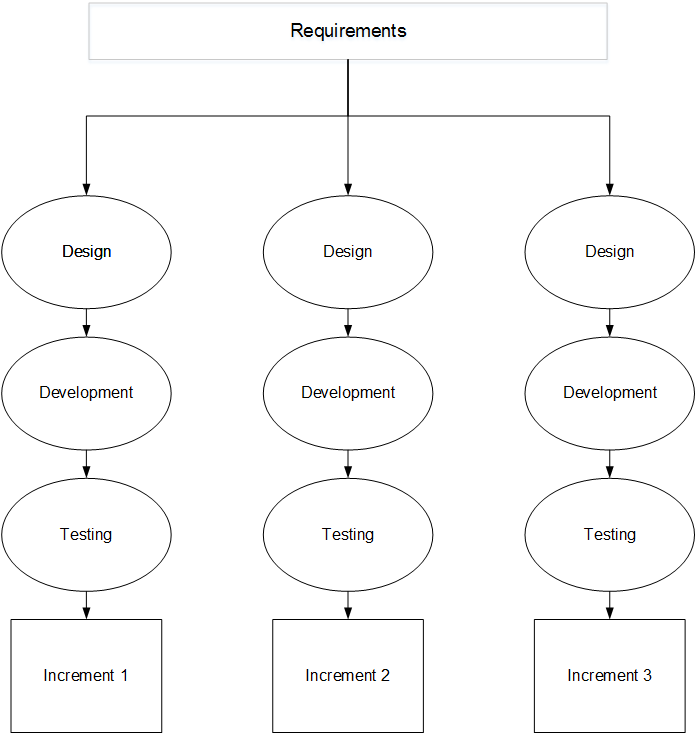
\includegraphics[width=1.0\textwidth]{Chapter3/Figs/Figure3-1.png}
    \caption[Iterative and incremental model]{Iterative and incremental model}
    \label{fig:Iterative and incremental model}
    \end{figure}
    
By using this method, the proposed authentication system was initiated through the use of a detailed planning process that involved mapping out the various goals for each increment of development. The goals for each increment included appending functionality to the previous increment. It was determined early on that by reaching these smaller goals and ensuring that the system functionality for each increment was met, the final system integration would be simplified. The holistic approach is important when developing a system using multiple increments. Due to the nature of the requirements that were set out in the early stages of research, the final authentication system would have to be constructed. As indicated in Chapter 2, various techniques are required to function as expected to in their own regular circumstances before they can be implemented, tested and integrated to the final system. 
The iterative and incremental model is one that is based on producing deliverables. To illustrate the planning that went into the development of this final system, Figure~\ref{fig:Requirements} is presented and discussed. 

% Figure - Requirements
    
    \begin{figure}[htbp!] 
    \centering    
    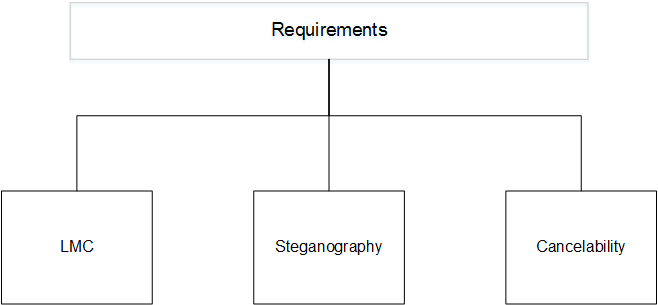
\includegraphics[width=1.0\textwidth]{Chapter3/Figs/Figure3-2.png}
    \caption[Requirements]{Requirements}
    \label{fig:Requirements}
    \end{figure}    
    
    The way in which the requirements for this project were setup and maintained was largely determined with the final system in mind. From the inception of this study, it was decided that the final authentication had to function in the following ways:
    
    \begin{enumerate}[label=\roman*.]
    	\item With the use of an inexpensive, functional peripheral device and an authentication sensor to provide a user-friendly and affordable solution to biometric readers;
    	\item The system would have to use a novel approach to storing biometric information obtained from the aforementioned sensor; and
    	\item Due to the novelty of the biometric storage, the system users’ biometrics should not be vulnerable to impersonation attacks.
    \end{enumerate}
    
With the functionality of the final authentication system established, the increments for the development phase became transparent. As seen in Figure~\ref{fig:Development life cycle for proposed authentication system}, the increments for the project would evolve around meeting three main requirements, namely:

    \begin{enumerate}[label=\roman*.]
        \item Use the leap motion controller as the authentication sensor and ensure that it can read user hands efficiently and accurately;
        \item Apply steganographic techniques as a storage mechanism for the biometric reading provided by the leap motion controller; and
        \item Ensure that the users original biometric readings are safely stored using the aforementioned CB techniques and that they are mathematically irreversible (as seen in Chapter 2).
    \end{enumerate}
    
   % Figure - Development life cycle for proposed authentication system
    
    \begin{figure}[htbp!] 
    \centering    
    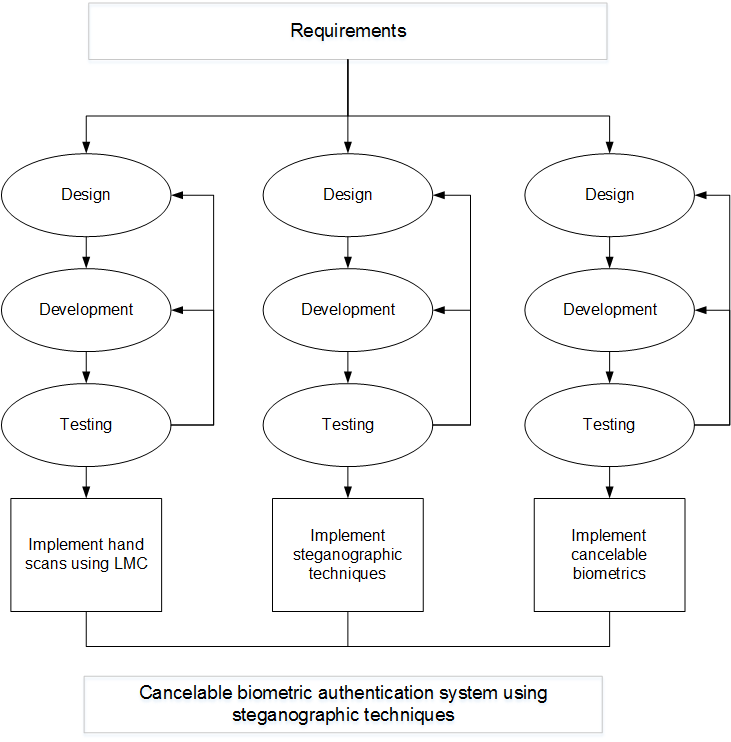
\includegraphics[width=1.0\textwidth]{Chapter3/Figs/Figure3-3.png}
    \caption[Development life cycle for proposed authentication system]{Development life cycle for proposed authentication system}
    \label{fig:Development life cycle for proposed authentication system}
    \end{figure}
    
	
The development process will be discussed in more detail regarding each increment and its iterations.
By using these requirements to guide the development process, the first increment was instantiated by attempting to learn how the leap motion controller can be used to extract more information regarding a user’s hand. For this, the developer documentation \footnote{https://developer.leapmotion.com/documentation/} was consulted regarding the setup thereof.

\section{Proposed framework}

The prevailing architectures of biometric authentication systems consist of two main phases. These phases involve enrolment and authentication. The reason these two phases are required is so that during the authentication phase, the system has a stored biometric to compare to the biometric currently being presented to the system. This comparative biometric is typically referred to as a biometric template. During the enrolment phase, the biometric template is created for the user and then stored in a database. The manner in which the biometric template is created consists of several images being taken of the hand and then algorithmically extracting features from those images to create a final model for the specified user ~\citep{Varchol2007}. This entire enrolment phase can be simplified through the use of an LMC due to its ability to extract hand features from the internal LMC hand model that is created upon presentation of the hand. In order to comply with CB practices, this hand model has its features transformed mathematically, such that the original biometric information is not used in the transit/storage processes. The authentication phase simply compares the presented hands’ extracted features to those of the models in the database. This authentication process would, therefore, also need to transform the presented biometrics in order to match it to the stored model.

Figure~\ref{fig:System structure flowchart} represents the information (system structure) flow in the authentication system. The LMC initiates the information flow for the system when the hand is presented and immediately extracts features therefrom. Once the features are extracted, they can be transformed mathematically allowing for the enrolment phase to commence. In an attempt to further secure the biometric information, the decision was made to implement two-factor authentication. This is done by issuing a four-digit PIN to each new user that is enrolled into the system. For implementation purposes, the use of four-digit PINs allows for a maximum unique user capacity of nine thousand users (randomly generated and numbered from 1000 to 9999). The issued user PIN will determine where in the stego-image the biometric information is stored. By taking this approach, the system is then able to use two different images for storage (one for PINs and one for the biometrics). 

% Figure - System structure flowchart
    
    \begin{figure}[htbp!] 
    \centering    
    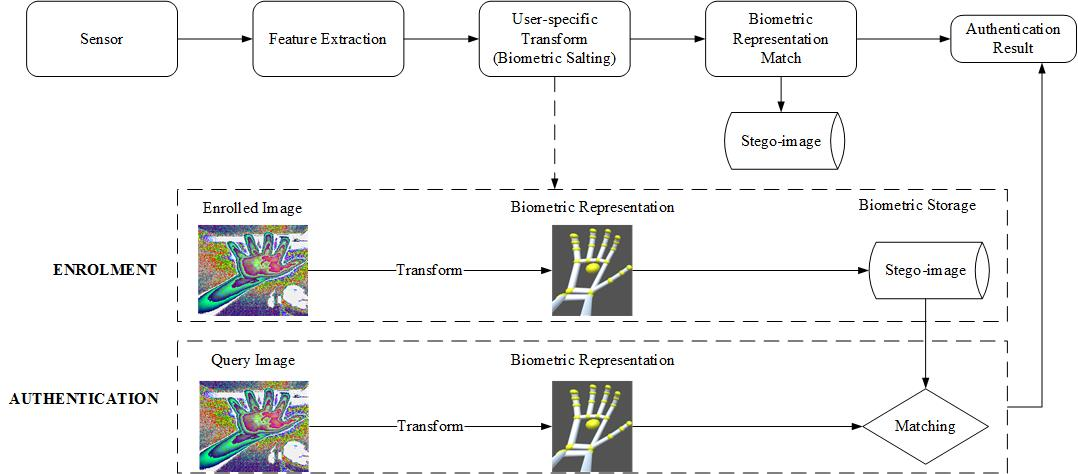
\includegraphics[width=1.0\textwidth]{Chapter3/Figs/Figure3-4.png}
    % \includesvg[width=1\textwidth]{Chapter3/SVG/Figure3-4.svg}
    \caption[System structure flowchart]{System structure flowchart}
    \label{fig:System structure flowchart}
    \end{figure}
    
In order to generate stego-images for sensitive information storage, one needs to specify exactly what images comprise of, how they are processed and how to programmatically generate them.

\section{System development process}

In the next section, an attempt is made to outline the process that was followed throughout the development of the proposed framework for the biometric authentication system. This is based on the objectives mentioned in Chapter 1, as well as the iterations mentioned earlier in this chapter.

\subsection{Development using the Leap Motion Controller}

As seen in Figure~\ref{fig:System structure flowchart}, the overall system structure flow is initiated through the feature extraction through the use of a sensor. In this particular study, the sensor refers to the Leap Motion Controller. To successfully extract features from the user, the LMC needs to be set up according to the particular environment that will be used throughout the development. 

The environment chosen for the study was based on prior knowledge, the level of support documentation provided by Leap Motion and available resources in order to minimise the amount of time taken to learn and adapt to novelties. 

\subsubsection{Leap Motion Controller development environment}

In order to reiterate the manner in which the LMC functions, one should refer to the API documentation for reference. For the purposes of feature extraction regarding the peripheral device, the hand detection can be summarised as follows:

Distance recorded by the LMC is measured in millimetres. 
To successfully extract accurate measurements pertaining to each individual hand that is presented to the LMC a Cartesian coordinate system is employed. 	This particular coordinate system manages to specify the various planes associated to the X-, Y- and Z-axis with regard to their orientation relative to the LMC device. This can be seen in Figure~\ref{fig:LMC device structure and orientation}\footnote{https://developer-archive.leapmotion.com/documentation/csharp/devguide/Leap-Overview.html}. 

% Figure - Randomly generated image versus stego-image
    
    \begin{figure}[htbp!] 
    \centering    
    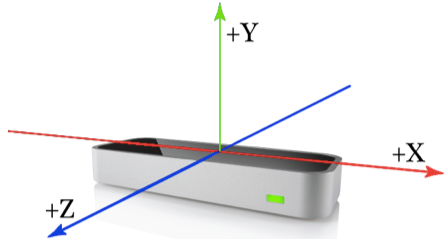
\includegraphics[width=1.0\textwidth]{Chapter3/Figs/Figure3-5.png}
    % \includesvg[width=1\textwidth]{Chapter3/SVG/Figure3-5.svg}
    \caption[LMC device structure and orientation]{LMC device structure and orientation}
    \label{fig:LMC device structure and orientation}
    \end{figure}


The LMC generates infrared light, along with the use of optical sensors that originate directly from the centre, on top of the device. The Y-axis directs the sensors upwards and provides values that are incremented positively, contrasting to the downward orientation of the majority of computer graphics coordinate systems. The X- and Z-axis lie on the horizontal plane of the LMC device with the X-axis positioned along the horizontal face of the device. The Z-axis provides positive values that increment toward the user. 

To provide further context as to how the LMC will be used to extract useful biometric information relating to the presented user hand, the following architecture allows a visual representation of the measurements that will be extracted during a scan. It is important to note that the LMC is capable of extracting far more information than what will be used in this particular study. The information and measurements relevant to this study include (and are limited to) the following information that can all be obtained from within the hand object. The hand object can further drill down into finger objects. These finger objects can then provide more information depending on the finger type. Each finger type then provides bone objects that list the bone type correlating to the specific finger type. From those bone types, one is then able to measure those particular bones.  As provided by the developer API documentation on Leap Motion’s website, Figure~\ref{fig:LMC presented hand objects during extraction} \footnote{https://developer-archive.leapmotion.com/documentation/csharp/devguide/Leap-Overview.html} provides a visual representation of how the hand object can be matched to suit the needs of this study.

% Figure - Randomly generated image versus stego-image
    
    \begin{figure}[htbp!] 
    \centering    
    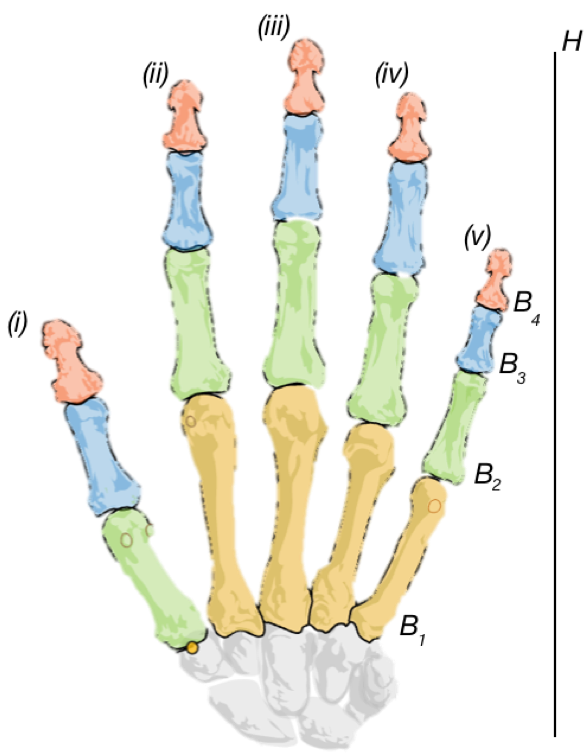
\includegraphics[width=8cm,height=9cm,keepaspectratio]{Chapter3/Figs/LMC_presented_hand_objects_during_extraction.png}
    \caption[LMC-presented hand objects during extraction]{LMC presented hand objects during extraction}
    \label{fig:LMC presented hand objects during extraction}
    \end{figure}

In Figure~\ref{fig:LMC presented hand objects during extraction}, it is relevant to present the corresponding information relating to the objects.

%  Table - LMC hand object mapping according to infrared scan


    \begin{table}[h!]
    \caption{LMC hand object mapping according to infrared scan}
    \centering
     \begin{tabular}{|p{0.3\textwidth} | p{0.3\textwidth}| p{0.3\textwidth}|} 
     \hline
    	\textbf{Object} & \textbf{Symbol} & \textbf{Name} \\ [1ex] 
     \hline\hline 
     Hand & \textit{H} & Hand Class  \\
     \hline 
     \multirow{5}{*}{Finger} & \textit{(i)} & Thumb \\

            & \textit{(ii)} & Index     \\
     
            & \textit{(iii)} & Middle     \\
     
            & \textit{(iv)} & Ring     \\
     
            & \textit{(v)} & pinkie      \\
    \hline        
    \multirow{4}{*}{Bone} & \(B_1\) & Metacarpal\\
     
            & \(B_2\) & Proximal phalanges     \\
     
            & \(B_3\) & Intermediate phalanges     \\
     
            & \(B_4\) & Distal phalanges     \\
     \hline
     \end{tabular}
    \end{table}
    
With the guidance of the API documentation provided by Leap Motion, it is possible to classify all the necessary information into a model that is easier to understand during the development process. 

With the use of the above table, it was evident what the class hierarchy would have to be in order to successfully implement the extraction of hand geometry measurements. The information would then be further classified using a Unified Modelling Language to visualise the object structure to be used in the extraction algorithm. Figure \ref{fig:UML object structure} represents the proposed object structure.

% Figure - UML
    
    \begin{figure}[htbp!] 
    \centering    
    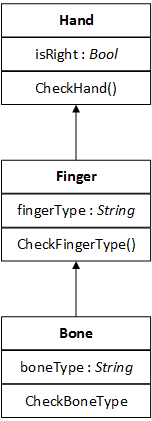
\includegraphics[width=8cm,height=9cm,keepaspectratio]{Chapter3/Figs/Object_Diagram.png}
    \caption[UML object structure]{UML object structure}
    \label{fig:UML object structure}
    \end{figure}

Once the model has been set out and the measurements have been extracted from the presented user hand one can then prepare the extracted biometric for transformation. However, prior to transformation, where the biometric will be stored and what the template will be must be considered, for this preparation for storage is done using steganographic techniques. In the following section, the stego-images and how they were generated will be discussed.

% \renewcommand{\umltextcolor}{black}
% \renewcommand{\umldrawcolor}{black}
% \renewcommand{\umlfillcolor}{white}

% \begin{center}
% \begin{tikzpicture}

% \begin{class}{ Hand }{0 ,0}
%     \attribute{ isRight : Bool }
%     \operation{ CheckHand (  )}
% \end{class}

% \begin{class}{ Finger }{ 0 , -5}
%     \inherit{ Hand }
%     \attribute{ fingerType : String }
%     \operation{ CheckFingerType ( )}
% \end{class}

% \begin{class}{ Bone }{0 , -10}
%     \inherit{ Finger }
%     \attribute{ boneType : String }
%     \operation{ CheckBoneType ( ) }
% \end{class}

% \end{tikzpicture}
% \end{center}


To aid the development process, Leap Motion has presumed the thumb metacarpal to have a length of 0.
These processes all occur at the time of initiating the scan via the LMC. To further illustrate the function used in the development of the extraction process, the following Algorithm~\ref{alg:Leap_motion_controller_algorithm_to_extract_hand_geometry} can be consulted.
    


%******************************************************************************************

% Algorithm - Leap motion controller algorithm to extract hand geometry

\begin{algorithm}[H]
 \SetKwInOut{Input}{Input}
    \SetKwInOut{Output}{Output}

    \underline{function ExtractHandGeometry} $(hand)$\;
    \Input{Hand object}
    \Output{Hand Measurements ($fingerLength$, $boneLength$)}
    \For{$hand$ in $hands$}{
        \eIf{$hand$=$RightHand$}{
            \For{$finger$ in $Fingers$}{
                \DontPrintSemicolon
                \space
                $fingerType$ = ClassifyFinger($finger$); 
                \tcp{Thumb, Index, Middle, Ring \& pinkie}
                
                \Switch{$fingerType$}{
                    
                
                    \For{$bone$ in $finger$}{
                        $boneType$ = ClassifyBoneType($finger$);
                        
                        \Switch{$boneType$}{
                            \tcp{Metacarpal, Proximal, Intermediate \& Distal }
                                AddMeasurements($boneType$);
                            
                        }
                    }
                }
                     
            }
            return $HandGeometryMeasurements$;
          }
          {
            return $CloseConnectionError$;
          }
    }
    \caption{Leap motion controller algorithm to extract hand geometry}     
    \label{alg:Leap_motion_controller_algorithm_to_extract_hand_geometry}
\end{algorithm}



To explain Algorithm~\ref{alg:Leap_motion_controller_algorithm_to_extract_hand_geometry}, the first check that has to be done is one to determine which hand it is. Once the hand is confirmed to be the right hand, the algorithm can then proceed to check the fingers of that hand. Upon classification of the finger, the bones of that finger are then checked. Upon classification of the bone type, within the finger, within the hand, the measurement can be stored in a list. This process occurs for each hand upon enrolment of the finger (prior to storage) and upon authentication to match the measurements.

This research includes the use of the technique of creating cancelable biometrics. The first transformation of the hand geometry occurs in the scan of the hand, whether it be during enrolment or authentication. What is done to the original measurement initiates the cancelability. During the initial ten second enrolment scan, the measurements are extracted as previously discussed in Algorithm~\ref{alg:Leap_motion_controller_algorithm_to_extract_hand_geometry}. However, before storage, all the measurements that have temporarily been stored in a list are then aggregated for each of the nineteen bones. This total is then divided by the number of measurements that were taken by the LMC during the scan. The average measurement for each bone is then stored in an array of nineteen unique measurements that are rounded off to the nearest integer. This array of nineteen measurements is then transformed for the first time into a vector of five unique values (one for each finger). This vector is five values and is the first line of defence in protecting the users biometric. The manner in which Algorithm~\ref{alg: Transform algorithm} protects the user's biometrics has to do with the transformation that takes place to form this new five value vector. For this example, the values are mathematically transformed by simply aggregating the bone measurements in each finger. It should be noted that any mathematical function can be applied at this point, however, for simplicity, the values are merely aggregated. 

Another technique can be applied at this point to practice cancelability, namely by simply discarding particular bone measurements ensures that the cancelability is reusable (as mentioned in Chapter 2). By simply changing the way in which the measurements are transformed, value can be added mathematically to ensure cancelability. 

An illustrative example will clarify this process towards the end of this section.\\

%******************************************************************

Algorithm~\ref{alg:Leap_motion_controller_algorithm_to_extract_hand_geometry} adds every user's hand geometry measurements to a list. This list consists of +-10 000 readings.

Once these readings have been recorded and stored during the initial scan, Algorithm~\ref{alg: Create user hand geometry during enrolment} is used to drill-down into meaningful hand geometry measurements. Algorithm~\ref{alg: Create user hand geometry during enrolment} is depicted below.

For each of the bones, in each of the fingers, on each of the hands, the measurements are aggregated. Once the measurements for each finger and it's bones are extracted, this Algorithm~\ref{alg: Create user hand geometry during enrolment} iterates through the stored readings, aggregates the values, calculates the average (aggregated readings/number of readings), rounded off to the nearest integer. Once this vector is created, the vector is then further transformed. 

%Algorithm - Create user hand geometry vector during enrolment

\begin{algorithm}
     \SetKwInOut{Input}{Input}
    \SetKwInOut{Output}{Output}
    \underline{function EnrolUser} $(HandGeometryMeasurements)$\;
    \Input{All of the different hand geometry measurements (Finger and Bone Lengths)}
    \Output{HandGeometry vector}
    
    $counter$; 
    
    $measurementAverages$; 
    
    \For{$value$ in $measurements$}{
        $measurementAverage$ += value;
    }
    $measurementAverage$ = \textit{RoundToNearestInteger($measurementAverage/counter$)};
    
    \For{$measurementAverage$ in $HandGeometryMeasurements$}{
    
        $vector$ = \textit{ArrayOfMeasurements($measurementAverage$)};
        
    }
    \tcp{Transformed vector from the array of measurements, passed through the final \textit{transformVector} function}
    
    
        $transformedVector$ = transformVector($vector$);
    return $transformedVector$
    \caption{Create user hand geometry vector during enrolment}
    \label{alg: Create user hand geometry during enrolment}
    
\end{algorithm}


\subsection{Steganographic development}

%Algorithm - Create stego-image for PINS

\begin{algorithm}
     \SetKwInOut{Input}{Input}
     \SetKwInOut{Output}{Output}
     
     \underline{function CreatePINStegoImage} ()\;
     \Output{$randomImage$}
     
     \textbf{Array} $allPins$ = \textbf{CreateUserPins(9 000)}\;
     
     \For{$pin$ in $allPins$}{
        GenerateHash($pin$)\;
     }
     
     \textbf{int} $length$ = $allPins$.Length\;
     
     $height$ = 90\;
     $width$ = 800\;
     
     Bitmap $randomImage$ = new Bitmap($width$, $height$)\;
     
     \For{(\textbf{int} y = 0; y < $height$; y++)}{
     
        \For{(\textbf{int} x = 0; x < $width$; x++)}{
        
            \For{\textbf{int} i = i < $length$; i += 4}{
            
                $a$ = $allPins$[i]\;
                $r$ = $allPins$[i + 1]\;
                $g$ = $allPins$[i + 2]\;
                $b$ = $allPins$[i + 3]\;
                
                $randomImage$.SetPixel(x, y, ARGB($a$, $r$, $g$, $b$))\;
            }
        
        
        }
     
     }
     
     return $randomImage$.Save()\;
     
     \caption{Create stego-image for PINs}
     \label{alg: Create stego-image for PINs}
\end{algorithm}

%******************************************************************
    %Create stego PIN image explanation
%******************************************************************
First and foremost to note was how pixels store information. The main concept behind working with pixels was the manner in which the data would be stored in the image in order to accurately represent a user’s hand geometry, while maintaining the privacy thereof. 

In order for this particular system to work, it had to be thoroughly planned and mathematically accurate to avoid any complications. With the original plan being to use multifactor authentication with the use of four-digit PINs, the manner in which these PINs are stored had to remain consistent and secure. Not only would the PINs have to be stored using steganography, but all of the users hand geometry that corresponded to each of those PINs as well. 

It was decided to incorporate a type of mapping technique that would have two separate stego-images. By mapping out the user PINs for both stego-images, it provided an easy way to map and keep track of the users and where their information was stored in the image. 

Initially, the random four-digit PINs needed to be generated and mapped to the corresponding pixels. The way this was done involved calculations that had to be tested and verified various times before the stego-images were successfully generated. 

Firstly, stego-image 1 would contain the random four-digit PINs after they had been hashed using the SHA-256 algorithm that was discussed in Chapter 2. The calculations went as follows:
The SHA-256 algorithm, as the name implies, produces a hash value consisting of 256bits. 
By using this algorithm for each of the PINs, one would have to specify what the bits per pixel (bpp) would have to be for each of the pixels in the stego-image. It was decided that 32bpp would be acceptable to use. This is due to the fact that the hashed values would suit this image format in terms of storage capacity.

Typically, what the bpp does is determine the number of colours that can be stored in an image. This number of colours in an image depends on the bpp value. This value grows exponentially. An example of this would be: 

If 1bpp is equal to two colours and 2bpp is equal to four colours, then 32bpp is equal to 4,294,967,296 colours. This is due to the stego-images using the format of 32bpp to store the hashed values in the A, R, G and B values (eight bits each).

Furthermore, as seen in Algorithm~\ref{alg: Create four-digit user PINs}, the values for the stego-images are generated at 90 X 800, providing a resolution of 7 200. This is simply because of the number of users who can have a unique four-digit PIN given to them of 9 000. This means that each users information will be mapped and stored to eight specific pixels in the stego-images. 

%******************************************************************

% Algorithm - Create four-digit user PINs

\begin{algorithm}
     \SetKwInOut{Input}{Input}
     \SetKwInOut{Output}{Output}
     
     \underline{function CreateUserPINs} ($numberOfUsers$)\;
     \Input{$numberOfUsers$}
     \Output{$userPins$}
     
     List $userPins$ \;
     
     \While{$numberOfUsers$ <= 9 000 \&\& !$userPins$.Contains()}
     {
        $userPins$.Add(Random(1 000, 10 000))\;
        $numberOfUsers$++\;
     }
     
     return $userPins$\;
     \caption{Create four-digit user PINs}
     \label{alg: Create four-digit user PINs}
     
\end{algorithm}

%******************************************************************
    %create 4 digit PIN explanation
%******************************************************************
The importance of generating the four-digit PINs randomly and assigning the users with these PINs is to provide better suited mapping capabilities. If this system were to be scaled, it could easily be done by simply generating five-digit PINs which would take the total number of users that the system could handle from 9 000 to 90 000.
\pagebreak
When generating the four-digit PINs that will be allocated to the users it is imperative that the following criteria are met:

\begin{enumerate}[label=\roman*.]
    \item No repeating PINs;
    \item 9 000 unique PINs are generated;
    \item Unordered sequence (pseudo-random); and
    \item PINs are only generated once.
\end{enumerate}





Due to the above-mentioned criteria, the PINs carry larger weight when applying them as multifactor authentication to the user along with his/her biometric. 

As described above, to meet the criteria for the PINs, it was decided to use PINs that start with 1. By doing so the number of PINs decreases from a possible 10000 to 9 000. 

The number of unique PINs can be verified using the following formula:
\begin{gather}
    N =  x^{n}    
\end{gather}


Where x is the number relating to the range of possible values that are considered. In this instance it would be 0 – 9, therefore x = 10. However, because this study is only considering values that start with 1 and upward, the formula can be rewritten as follows:

\begin{gather}
    N = a^{n}.b^{n}.c^{n}.d^{n}    
\end{gather}


Where N is the number of possible unique values and a, b, c and d are the positions in the four-digit PIN. In this particular example, a only has 9 possible values ranging from 1 to 9, whereas b, c and d can range from 0 to 9. This produces the equation:

\begin{gather}
    N = 9^{1}.10^{1}.10^{1}.10^{1} 
    = 9 000    
\end{gather}



To calculate the probability of another user being able to guess your PIN, one would need to look at the statistical formula: 
\begin{gather}
    P (A) = \frac{NumberOfFavourableOutcomes}{TotalNumberOfPossibleOutcomes}
\end{gather}


Where the probability of event A in this instance is 
\begin{gather}
    \frac{1}{9 000} = 0,000111111.
\end{gather}

With the probability as low as this enhanced by the biometric feature transformation added to it, the likelihood of guessing a PIN and matching the biometric is very close to zero.

%******************************************************************
%Algorithm -  Create stego-image for users

\begin{algorithm}
     \SetKwInOut{Input}{Input}
     \SetKwInOut{Output}{Output}
     \underline{function CreateUserStegoImage} ($bitmap$, $bytes$)\;
     \Input{$bitmap$}
     \Output{$userAddedBitmap$}
     \tcp{Depending on the x, y coordinates associated to pin}
     \eIf{$bitmap$.GetPixels(x,y) == \textbf{populated}}{
        return Error\;
     }{
        \For{(\textbf{int} i = 0; i < 32; i += 4 )}{
        $userAddedBitmap$ = $bitmap$.SetPixel(x, y, ARGB($bytes$[i], $bytes$[i + 1], $bytes$[i + 2], $bytes$[i + 3]))\;
        }
     }
     return $userAddedBitmap$
     \caption{Create stego-image for users}
     \label{alg: Create stego-image for users}
     
\end{algorithm}

%******************************************************************
    %create stego-image 2 explanation
%******************************************************************

Initially, stego-image 2 is generated as a blank image with zero values for each pixel. The resolution of stego-image 2 is required to stay consistent with that of stego-image 1 in order to ensure uniformity during the enrolment and authentication phases. Algorithm~\ref{alg: Create stego-image for users} occurs during the enrolment phase where admin rights should be displayed in order to add a user to the system. Upon enrolment, the system will allocate a PIN to the user. Once the PIN has been allocated to the user, the system will then attempt to populate the transformed geometry into the eight pixels that are mapped in the same position of the PIN in stego-image 1. General error checking is shown in Algorithm~\ref{alg: Create stego-image for users}, but due to the transformed hand geometry being hashed using SHA-256, the bytes will be set accordingly into the specified pixels. When the user attempts to authenticate using the system, another scan will occur, the hand geometry will be transformed once more and then matched according to the new hash value.

\subsection{Stego-image contextualisation}

An abstraction of what an image can be seen as is a two-dimensional matrix that is made up of pixels containing information about the colours in each particular pixel. This pixel information can be used to store sensitive biometric information. Using steganography techniques to store the transformed biometric models in an image involves that in order to store these models, each model's bit data would have to be processed. All electronic information is essentially made up of 1’s and 0’s (or bits). This means that the models that are generated need to be manipulated in such a manner that each user model’s bit data can be extracted for processing thereof. Once this bit data is processed, it can then be stored in an image to correspond to a particular user. 

With two-factor authentication being applied, both the PIN and the hand geometry need to be stored. Using one image to store the PIN, the system can then use the stored PIN to enrol/locate a user in a second image. This can be likened to a one-to-one relational database model. To illustrate this concept, Table II shows how PIN information in the first image can be used to correspond to the hand geometry stored in the second image. For instance, in the first block of Table II, the bold number (1) represents the user ID slot number while 3648 is the user PIN. The corresponding slot in the second stego-image is then used as the storage location for the user hand geometry data.

%  Table - Stego-image 1: User IDs vs their pixel correlation (10 IDs x 8 pixels per ID x 5 rows


    \begin{table}[h!]
    \caption{Stego-image 1: User IDs vs their pixel correlation (10 IDs x 8 pixels per ID x 5 rows}
    \centering
     \begin{tabular}{|p{0.075\textwidth} | p{0.075\textwidth}| p{0.075\textwidth} | p{0.075\textwidth} | p{0.075\textwidth} | p{0.075\textwidth} | p{0.075\textwidth} | p{0.075\textwidth} | p{0.075\textwidth} | p{0.075\textwidth} |} 
     
     \hline
     \begin{minipage}{.075\textwidth}
      
\includegraphics[width=\linewidth, height=5mm]{Chapter3/Figs/TablePixels.jpg}
    \end{minipage}& & & & & & & & & \\[1ex]
     \textbf{1}, & \textbf{2}, & \textbf{3}, & \textbf{4}, & \textbf{5}, & \textbf{6}, & \textbf{7}, & \textbf{8}, & \textbf{9}, & \textbf{10},  \\[1ex]
     3648 & 7896 & 5091 & 4948 & 3102 & 7500 & 1651 & 6765 & 6865 & 7677  \\[1ex]
     
     \hline 
     \textbf{11}, & \textbf{12} & \textbf{13} & \textbf{14}, & \textbf{15}, & \textbf{16}, & \textbf{17}, & \textbf{18}, & \textbf{19}, & \textbf{20},  \\[1ex]
    5153 & 1782 & 2922 & 2183 & 1817 & 6372 & 1621 & 8283 & 2845 & 6931  \\[1ex]
     
     \hline
     \textbf{21}, & \textbf{22}, & \textbf{23}, & \textbf{24}, & \textbf{25}, & \textbf{26}, & \textbf{27}, & \textbf{28}, & \textbf{29}, & \textbf{30},  \\[1ex]
    2608 & 3587 & 6231 & 5373 & 3594 & 1877 & 3867 & 1080 & 2807 & 6143  \\[1ex]
     
     \hline           
     \textbf{31}, & \textbf{32}, & \textbf{33}, & \textbf{34}, & \textbf{35}, & \textbf{36}, & \textbf{37}, & \textbf{38}, & \textbf{39}, & \textbf{40},  \\[1ex]
     7362 & 4162 & 8075 & 8742 & 7851 & 3653 & 8431 & 4352 & 1238 & 2128  \\[1ex]
     
     \hline
     \textbf{41}, & \textbf{42}, & \textbf{43}, & \textbf{44}, & \textbf{45}, & \textbf{46}, & \textbf{47}, & \textbf{48}, & \textbf{49}, & \textbf{50},  \\[1ex]
    7673 & 2513 & 8825 & 5110 & 5701 & 6623 & 5963 & 1703 & 3697 & 2073  \\[1ex]
     
     \hline
     
     \end{tabular}
    \end{table}
    


%******************************************************************************************

In order to standardise the amount of data that can be used to store information in the pixels, the system uses 32bpp (bits per pixel) image formatting. This ensures that in each pixel of the image, 32 bits of information can be held. These 32 bits are made up of A (eight bits), R (eight bits), G (eight bits), and B (eight bits) values. Due to the fact that the number of bits used to store a four-digit PIN would vary depending on the value, it was decided to also standardise the number of bits used during PIN storage per user. To do so, a hash-function is used \citep{Kashyap2016}. 
The hash-function ensures that regardless of what the PIN is, the length of the hash representation will be similar. A SHA256 (Secure Hashing Algorithm 256-bit) function was chosen. This is because it is the successor of SHA1, which was compromised \citep{Brandom}, and addresses the issues prevalent in SHA1.
Each PIN is made up of 256-bits (eight pixels, if one pixel = 32bpp), leading to eight pixels to store user their information in both images. Referring back to the earlier statement of using two images with a one-to-one relationship, a user PIN can be mapped and correlated directly to the hand geometry in the second image using the hash function prior to enrolling the user.

Table II is an example illustration of user ID slots in correlation to the image pixels with an image resolution of 80 X 5. The first image is used to store hashed user PINs. 
To generate the stego-image, the PINs are shuffled to ensure that the PIN-ID combination is not sorted in such a manner that PIN 1 000 is stored in the first eight pixels using the ID slot 1, etc.

\subsection{Random PIN generation}

To counter the threat of reverse engineering the generated PINs, 9 000 (unsorted) unique four-digit PINs were generated and each PIN mapped to an ID that ranged from 1-9 000. An example of such a mapping is demonstrated using Table II to illustrate that PIN 3648 correlates to the user ID of 1. With this information generated and stored locally, using a conversion to bit data, stego-image 1 was generated so that all of the hashed PINs were stored and mapped. Stego-image 1 will thus remain unaltered after it has been generated. Stego-image 2 can then be altered during the enrolment phase. This is further explained below.

\subsection{Stego-image generation}

Stego-image 2 is a randomly generated image that will be altered as users enrol into the system. During the enrolment phase, users will be issued a PIN. Depending on the PIN he/she receives, a user ID correlating to that PIN is known by the system. Once the system has calculated the user ID based on the PIN that was entered by the user, the pixels in stego-image 2 can be altered using the hashed hand geometry of the enrolling user. By altering stego-image 2 in this way using stego-image 1, the authentication phase become more efficient because the pixels containing the biometric information can be directly read due to the mapping. The authentication process would be inefficient if the system had to search through the entire image each time a user presented his/her hand. Since an image can be seen as a matrix with 9 000 users, the complexity to compare and authenticate the presented hand geometry to the image would be O(n²) each time. 

In order to gain a better understanding of how the system operates, the pseudo-code for the system is subsequently discussed.

\subsection{Cancelable biometric development}

The SHA-256 algorithm was discussed in detail in Chapter 2. However, it has been revisited here in Algorithm~\ref{alg: Generate hash algorithm} for completeness in order to provide context for how the bytes will be stored in the stego-images.

What Algorithm~\ref{alg: Generate hash algorithm} does is prepare the transformed vector for storage in stego-image 2 by returning bytes of data that are irreversible and safely secured.

%Algorithm - Generate Hash Algorithm
\begin{algorithm}
     \SetKwInOut{Input}{Input}
     \SetKwInOut{Output}{Output}
     
     \underline{function GenerateHash} ($transformedVector$)\;
     \Input{$transformedVector$}
     \Output{$vectorHash$}
     
     \textbf{\textit{using} SHA-256}{
        $hash$ = ComputeHash($transformedVector$)\;
        
        \For{$byte$ in $hash$}{
            $vectorHash$.add($byte$)\; 
        }
    
     }
     return $vectorHash$;
     \caption{Generate hash algorithm}
     \label{alg: Generate hash algorithm}
     
\end{algorithm}

The transformed vector that is passed into this function comes in the form of a text representation subsequent to the extraction scan that takes place from the LMC device. This will be further demonstrated in the following section that discusses the illustrative example. However, Algorithm~\ref{alg: Transform algorithm} revisits the simple transformation that occurs after the hand has successfully been scanned by the LMC and the measurements have been extracted. 

%Algorithm - Transform algorithm

\begin{algorithm}
     \SetKwInOut{Input}{Input}
     \SetKwInOut{Output}{Output}
     
     \underline{function TransformVector}($ArrayOfMeasurements$)\;
     \Input{$ArrayOfMeasurements$}
     \Output{$transformed vector$}
     
     \For{$measurementAverage$ in $ArrayOfMeasurements$}{
        $transformedVector$ += $measurementAverage$\; 
        \tcp{Aggregated measurements for this example} 
     }
     
     return $transformedVector$\;
     \caption{Transform algorithm}
     \label{alg: Transform algorithm}
     
\end{algorithm}




%******************************************************************
    %generate hash output explanation
%******************************************************************




\subsection{Pseudocode for system algorithm}

Keeping the above-mentioned information flow, as well as the mapping and stego-image generation in mind, this pseudocode should verify the exact functioning of the authentication system. 
The pseudocode below (Algorithm~\ref{alg: Pseudocode for system algorithm}) aims to provide an overview of what input is retrieved in the system and to clarify how the two phases of biometric systems are applied based on the input retrieved from the user. As seen above, if the user is enrolled, the system merely transforms the presented hand geometry and authenticates the user by comparing the transformed information to that stored in stego-image 2.

%  Algorithm - Pseudocode for system algorithm

\begin{algorithm}
     \SetKwInOut{Input}{Input}
     \SetKwInOut{Output}{Output}
     
     \underline{function cancelableTransform($PIN$, array[] $fingerBoneInfo$)}\;
     \Input{$PIN$, $Biometric Features$ {handID (hID), array[boneType (bT), boneWidth (bW), boneLength (bL)]}}
     \Output{User-specific HashID for Steganography}
     
      \eIf{(PIN == hID) \&\& (enrolled == true)}{
        handGeo = Transform(fingerBoneInfo)\;
        Authenticate(getPixels(map),handGeo)\;
      }{
        newUser = Transform(fingerBoneInfo)\;
        EnrolUser(PIN, newUser)\;
      } 
        
      return HashID\;
     \caption{Pseudocode for system algorithm}
     \label{alg: Pseudocode for system algorithm}
     
\end{algorithm}

%*********************************************************

%******************************************************************
    %pseudocode explanation
%******************************************************************

The pseudocode for the entire system algorithm attempts to summarise the process that the authentication system follows, from the initial scan during enrolment to the matching the transformed biometric that is presented by the user during authentication.

Algorithm~\ref{alg: Pseudocode for system algorithm} describes the logic behind the system in a simplified manner to portray the main functionality. 

%******************************************************************


However, if the user has not been enrolled, he/she is then issued a PIN and the presented hand geometry is transformed and stored in stego-image 2, correlating to the issued PIN location.

Next, the advantages and disadvantages of the system will be discussed.

\subsection{Discussion}

The use of the current implementation of this authentication system has its advantages and disadvantages.


Advantages of the proposed system include:
    \begin{enumerate}[label=\roman*.]
        \item The low-cost factor; 
        \item Ease of use and convenience;
        \item The security aspects are superior when compared to passwords because authentication is based on a combination of PIN and hand information that cannot be stolen or guessed; and
        \item Auditability in terms of being able to connect users to a specific event or activity.
    \end{enumerate}
	
The disadvantages include: 
    \begin{enumerate}[label=\roman*.]
        \item The technology is still in its infancy and is not mature;
        \item While system performance for authentication is expected to be high for small organisations, it may pose a problem should more users need to be enrolled; and
        \item Error incidence due to changes in a person’s hands due to injury, old age, or illness.
    \end{enumerate}

The following section will provide an illustrative example of the system.

\section{Illustrative example}

In this section, a simplified example of a user being authenticated is presented in order to provide a holistic view of the combination of the topics discussed in previous sections.
With each hand that is presented to the LMC a model is created that is either used for enrolment or for authentication. Assuming that the user hand that is presented has already undergone enrolment, the LMC will create a model using a particular transform parameter to compare this model to the binary representation of the hand already stored in stego-image 2. By using the PIN that is entered prior to hand scanning, the system ensures that the user's transformed biometric representation can efficiently be compared to the newly transformed model. This is efficient because the system has mapped the PINs to pixel IDs, rather than having to search the entire image for the corresponding biometric representation.

Consider the explanation of the illustrative example shown in Figure~\ref{fig:Example of biometric vector reading and transformation}.

% Figure - Example of biometric vector reading and transformation
    
    \begin{figure}[htbp!] 
    \centering    
    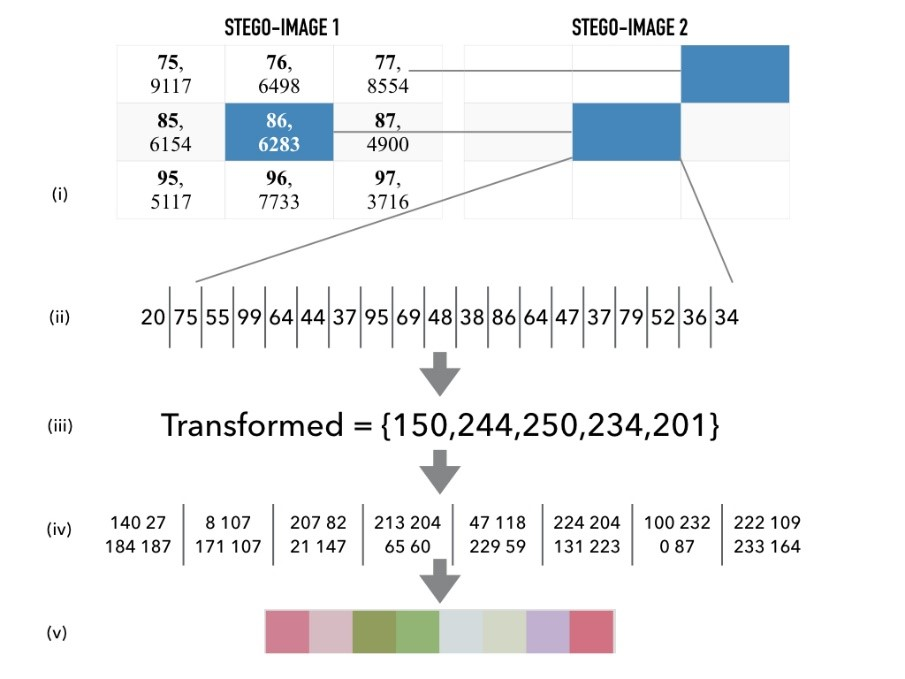
\includegraphics[width=1.0\textwidth]{Chapter3/Figs/Figure3-6.png}
    \caption[Example of biometric vector reading and transformation]{Example of biometric vector reading and transformation}
    \label{fig:Example of biometric vector reading and transformation}
    \end{figure}

\begin{enumerate}[label=\roman*.]
    
    \item  Assume the user was presented with the PIN 6283 during enrolment. The user would then have a dedicated storage section with the ID of 86 in both stego-image 1 and in stego-image 2. During the authentication phase the user will have his/her hand geometry scanned to compare the presented hand to the binary representation stored in stego-image 2. 
    
    \item  During the above-mentioned scan, the hand geometry of the user is mathematically generated by using various combinations from the thousands of readings gathered to form one vector (readings for each of the 19 individual bones in his/her hand).
    
    \item By using the vector created in (ii), the system then transforms the biometric vector once more in order to implement CB (as discussed in Section II-A). In this particular example, the vector was simply transformed by adding each finger’s bone readings together (three readings for the thumb and four readings for all the other fingers). It should be noted that more complex mathematical transformations are recommended for the actual implementation.
    
    \item The system further protects the biometric information by applying a SHA256 hash function to the vector. This vector is then represented as a byte array consisting of 32 values from the 256-bit hash function. Ultimately, this ensures that each user only uses eight pixels in both the stego-images.
    
    \item Once the byte array has been generated, it can then be compared to the stored biometric representation in ID 86 consisting of eight pixels.
Upon completion of the above-mentioned process, the system will either accept the user as successfully authenticated, or the system will reject the user and ask for the hand to be re-scanned.

\end{enumerate}

By using steganography techniques, the system ensures imperceptibility and cancelability.

Figure~\ref{fig:Randomly generated image versus stego-image} provides a comparative view of two generated images for their use in this context. 

% Figure - Randomly generated image versus stego-image
    
    \begin{figure}[htbp!] 
    \centering    
    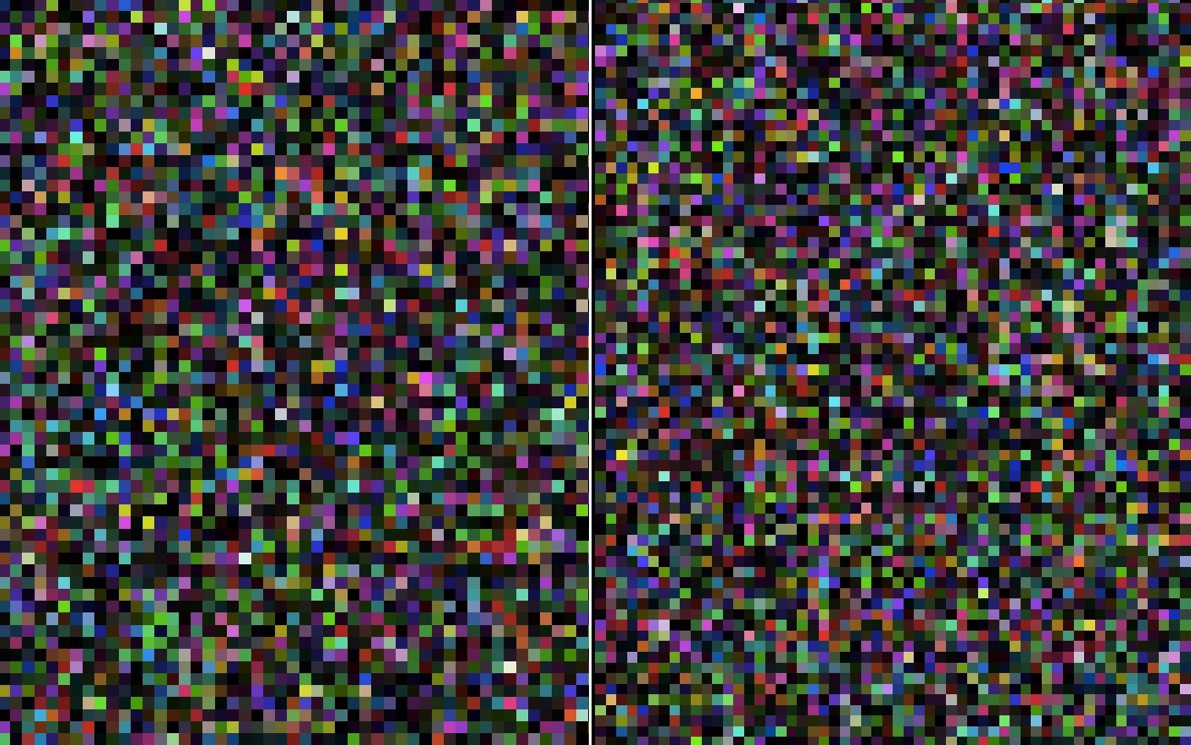
\includegraphics[width=1.0\textwidth]{Chapter3/Figs/Figure3-7.png}
    \caption[Randomly generated image versus stego-image]{Randomly generated image versus stego-image}
    \label{fig:Randomly generated image versus stego-image}
    \end{figure}

The image on the left was randomly generated, while the image on the right contains sensitive biometric information. To the human eye one cannot easily infer that these two images differ, however, upon closer inspection one may realise differing colour mappings but cannot differentiate between sensitive data and just another randomly generated image.

Ultimately, cancelability can be concluded due to the biometric information being transformed and obscured prior to storage. This means that should an attacker find these two images in a compromised system, he/she will not know what information was used to generate these images, nor how the information was transformed prior to storage. In fact, without prior knowledge he/she will not even know to expect hidden data in said images.

\section{Chapter summary}

The purpose of this chapter was to demonstrate the approach used throughout the system design and implementation thereof. Due to the system consisting of various iterations, the development of the system involved a considerable amount of integration. With the use of algorithms and an illustrative example, the functionality of the system (increments, as well as integrated) was thoroughly and explicitly explained in order to provide greater context. 

In Chapter 4, the results produced by the authentication system will be analysed, and the algorithmic performance and evaluation will be discussed.

